\documentclass[11pt,a4paper,oldfontcommands,oneside]{memoir}
\usepackage[utf8]{inputenc}
\usepackage{microtype}
\usepackage[dvips]{graphicx}
\usepackage{xcolor}
\usepackage{times}
\usepackage{graphicx}
\usepackage[spanish]{babel}

\usepackage[
breaklinks=true,colorlinks=true,
%linkcolor=blue,urlcolor=blue,citecolor=blue,% PDF VIEW
linkcolor=black,urlcolor=black,citecolor=black,% PRINT
bookmarks=true,bookmarksopenlevel=2]{hyperref}

\usepackage{geometry}
% PDF VIEW
% \geometry{total={210mm,297mm},
% left=25mm,right=25mm,%
% bindingoffset=0mm, top=25mm,bottom=25mm}
% PRINT
\geometry{total={210mm,297mm},
left=20mm,right=20mm,
bindingoffset=10mm, top=25mm,bottom=25mm}

\OnehalfSpacing
%\linespread{1.3}

%%% CHAPTER'S STYLE
\chapterstyle{bianchi}
%\chapterstyle{ger}
%\chapterstyle{madsen}
%\chapterstyle{ell}
%%% STYLE OF SECTIONS, SUBSECTIONS, AND SUBSUBSECTIONS
\setsecheadstyle{\Large\bfseries\sffamily\raggedright}
\setsubsecheadstyle{\large\bfseries\sffamily\raggedright}
\setsubsubsecheadstyle{\bfseries\sffamily\raggedright}


%%% STYLE OF PAGES NUMBERING
%\pagestyle{companion}\nouppercaseheads 
%\pagestyle{headings}
%\pagestyle{Ruled}
\pagestyle{plain}
\makepagestyle{plain}
\makeevenfoot{plain}{\thepage}{}{}
\makeoddfoot{plain}{}{}{\thepage}
\makeevenhead{plain}{}{}{}
\makeoddhead{plain}{}{}{}


\maxsecnumdepth{subsection} % chapters, sections, and subsections are numbered
\maxtocdepth{subsection} % chapters, sections, and subsections are in the Table of Contents

\begin{document}

\thispagestyle{empty}

{%%%
\sffamily
\centering
\Large

~\vspace{\fill}


\includegraphics[scale=1]{Escudo.png}\\
\vspace{50mm} %5mm vertical space
{\huge 
Describir las condiciones de singularidad de manipuladores seriales
}
\vspace{1.5cm}

{\LARGE
 Fonseca Camarena Jonathan
}

\vspace{3.5cm}

Universidad Politécnica de la Zona Metropolitana de Guadalajara

\vspace{3.5cm}

Profesor: Carlos Enrique Morán Garabito

\vspace{\fill}

Fecha de entrega, 1 de octubre del 2019

%%%
}%%%

\vspace{4.5cm}




\tableofcontents*

\clearpage

%%%---%%%---%%%---%%%---%%%---%%%---%%%---%%%---%%%---%%%---%%%---%%%---%%%
%%%---%%%---%%%---%%%---%%%---%%%---%%%---%%%---%%%---%%%---%%%---%%%---%%%

\chapter{Introducción}
Un manipulador serial se encuentra en una configuración singular cuando su órgano terminal es incapaz de moverse con una velocidad arbitraria dentro del espacio de trabajo. Esta situación es en general indeseable y debe evitarse o eliminarse. La primera opción es fácil de realizar aunque conlleva una reducción del espacio de trabajo. La mayoría de los manipuladores deben ser capaces de operar en configuraciones singulares. Si la singularidad es inevitable, es necesario implementar un procedimiento que permita eliminar la singularidad en que se encuentra el manipulador serial para tratar de recuperar su completa movilidad. 
\section{Singularidad}
Un robot manipulador presenta una configuración singular cuando el Jacobiano posee lineas que son linealmente dependientes. \\
Se llama SINGULARIDAD LIMITE cuando el manipulador está completamente distendido o retraído. \\
Se llama SINGULARIDAD INTERNA cuando ocurre el alineamiento de dos o mas ejes de los sistemas de coordenadas, tornando las lineas del Jacobiano linealmente dependientes. Este tipo de singularidad puede ocurrir en cualquier posición del actuador final. \\
Es importante conocer las configuraciones singulares del robot por las siguientes razones: Causa pérdida de movilidad del robot; Cuando el robot está en una configuración singular, pueden existir infinitas soluciones para la cinemática inversa; Cuando el manipulador se aproxima a una configuración singular, una pequeña velocidad del actuador final provoca grandes velocidades en el accionamento del robot.\\
\section{Configuraciones singurales (Jacobiano)}
Se denominan configuraciones singulares de un robot a aquellas en las que el determinante de su matriz Jacobiana se anula. Por esta circunstancia, en las configuraciones singulares no existe Jacobiana inversa. Al anularse el Jacobiano, un incrementó infinitesimal de las coordenadas cartesiana supondría un incremento infinito de las coordenadas articulares, lo que en la práctica se traduce en que en las inmediaciones de las configuraciones angulares, el pretender que  el extremo de robot se mueva a velocidad constante, obligaría a movimientos de las articulaciones a velocidades inabordable por sus actuadores.\\
Por ello, en las inmediaciones de las configuraciones singulares se pierde alguno de los grados de libertad del robot, siendo imposible que su extremo se mueva con una determinada dirección cartesiana. 
\section{Espacio de Trabajo}
El espacio de trabajo de un robot es la zona del espaciofísico que puede ser alcanzada por un punto de su órgano terminal. Lo anterior incluye el espacio cartesiano terminal.y las diferentes formas de expresar la orientación Euler, cuaterniones, etc.\\
Para determinar el espacio de trabajo se debenconsiderar las dimensiones de los eslabones, los limites en las articulaciones, y los diferentes tipos de singulares.\\
Además, se deben considerar manipulador las colisiones entre los eslabones del mismo manipulador.\\
El método geométrico consiste en analizarla geometría de los eslabones y el movimiento relativo que las articulaciones permiten realizar.\\
La discretizacion del espacio detrabajo consiste en definir una malla denodos para ser explorada.\\ Mediante unproceso interativo quee explora cada nodo para determinar si pertenece al espaciode trabajo o no.\\A través de este método se pueden considerara todas las restricciones posibles, como lo son los límites articulares, la colisión entre eslabones,y los diferentes tipos de singularidades.\\
Espacio de trabajo máximo (o alcanzable) está compuesto por todos los puntos en el espacio cartesiano que el efector final puede alcanzar con almenos una orientación.\\
Espacio de trabajo de traslación está compuesto por todos los posibles puntos en el espacio cartesiano que el efector final puede alcanzar en una orientación dada.\\
Espacio de trabajo de orientación se compone de todos las posibles orientaciones que se pueden alcanzar para una posición fija del efecto final.\\
Espacio de trabajo diestro está compuesto por todos los puntos en el espacio cartesiano que pueden ser alcanzados y en los cuales se puede alcanzar todas las orientaciones.\\
Espacio de trabajo diestro y controlable es un subconjunto del espacio detrabajo diestro que no contiene configuraciones singulares.\cite{angeles1992kinematic}

\section{Clasificación}
-	Singularidades en los límites del espacio de trabajo de robot. Se presentan con el extremo del robot esta en algún punto del límite del trabajo interior o exterior. En esta situación resulta obvio que el robot no podrá desplazarse en las direcciones que lo alejan de este espacio de trabajo.\\
-	Singularidades en el interior del espacio de trabajo del robot. Ocurren dentro de la zona de trabajo y se producen generalmente por el alineamiento de dos o más ejes de las articulaciones de robot.
\section{Aplicaciones}
1.Simuladores de vuelo (CAE)\\
2.Maquinado de piezas (Ingersoll) \\
3.Trasporte de objetos (Fanuc) \\
4.Posicionamiento de precisión (PI) \\
5.Medicina (UPM, U. de Tokyo) \\
6.Dispositivos hapticos(Falcon y Dispositivo de la Universidad MiguelHernández)\\
7.(IRRCyN IRRCyN).Vertebras de un robot anguila (IRRCyN)\\
8.Remo I es un robot submarino con una estructura paralela quepermite controlar laposición y orientación del impulsor con respecto con cabina. Remo I, UPM.\\



 
\section{Ejemplo}
Para el robot SCARA del que se obtuvo la matriz Jacobiana, se tiene que:
\begin{figure}[h]
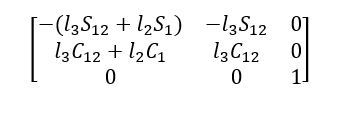
\includegraphics[scale=.9]{link1.png}
\end{figure}
Por lo que el Jacobiano será:
\begin{figure}[h]
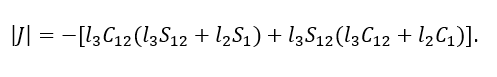
\includegraphics[scale=.9]{link2.png}
\end{figure}

Que se anula para:

\begin{figure}[h]
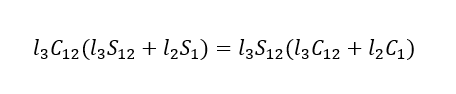
\includegraphics[scale=.9]{link3.png}
\end{figure}
Lo que se cumple siempre que q2=0 o pi, pues entonces la igualdad anterior se verifica para cualquier q1:
\begin{figure}[h]
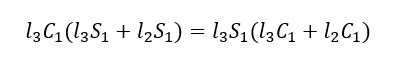
\includegraphics[scale=.9]{link4.png}
\end{figure}
Esta situación definida por q2=0 o pi corresponde a los puntos limites del espacio de trabajo del robot.\\
Q2 = 0: Limite exterior del espacio de trabajo.\\
Q2 = pi: Limite interior del espacio de trabajo.\\

Se debe prestar especial atención a la localización de las configuraciones singulares del robot para que sean tenidas en cuenta en su control, evitándose solicitar a los actuadores movimientos a velocidades inabordable o cambios bruscos de los mismos.\\
La figura muestra el resultado de intentar realizar con un robot tipo SCARA \ref{Imagen2}, una trayectoria en línea recta a velocidad constante que pasa por una configuración singular. Obsérvese la brusca variación de la velocidad articular q1 que crece hasta valores inalcanzables en la práctica.\cite{hayes2002singular}
\begin{figure}[h]
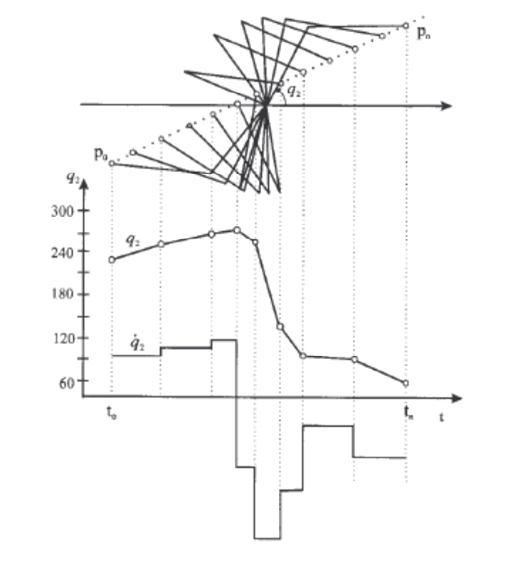
\includegraphics[scale=1.1]{link5.png}
\caption{Ejemplo}
\label{Imagen2}
\end{figure}
Un posible procedimiento para resolver la presencia de la singularidad interior al espacio de trabajo, en la que se pierde la utilidad de alguna articulación (pérdida de algún grado de libertad) sería el siguiente:\\
1.- Identificar la articulación correspondiente al grado de libertad perdido (causante de que el determinante se anule).\\
2.- Eliminar la fila de la Jacobiana correspondiente al grado de libertad perdido y la columna correspondiente a la articulación causante.\\
3.- Una nueva Jacobiana reducida (rango-1) obtener las velocidades de todas las articulaciones, a excepción de la eliminada, necesarias para conseguir las velocidades cartesiana preciadas. La velocidad de la articulación eliminada se mantendrá a cero.
\section{Condiciones}
Para poder obtener expresiones analíticas de las curvas límites (o superficies), basándose en el trabajo de Goyal and Sethi (2010), se deben seguir los siguientes pasos:\\
Definir la postura del efector final en términos de coordenadas generalizadas, es decir resolver la cinemática del robot.\\
Determinar las curvas (superficies) generadas por las singularidades.\\
Determinar el subset de esas curvas (superficies) debidas a los límites de las articulaciones.\\
Combinar todas las curvas (superficies) para representar el espacio de trabajo.\\
\cite{baturone2005robotica}
\section{Conclusión}
Según la investigación realizada, en las ultimas décadas se han utilizado robots Enparalelos para muy variadas aplicaciones.\\
•En esta investigación revisamos algunos de los Enconceptos mas importantes sobre el estudio de estetipo de robots.\\
•Actualmente encontrar mejores soluciones a los problemas deplanificación de trayectorias, determinación. evitaciónde singularidades, calibración, cinemática directa,control.
•Pero más imporntate es que nosotros entendamos la prespectica de cómo los planos van cambiando serialmente para que los calculos nos salgan correctamente.

\bibliographystyle{plain}
\bibliography{torres}


\end{document}

